\chapter{相關研究}
\label{章:相關研究}

\begin{figure}
\centerline{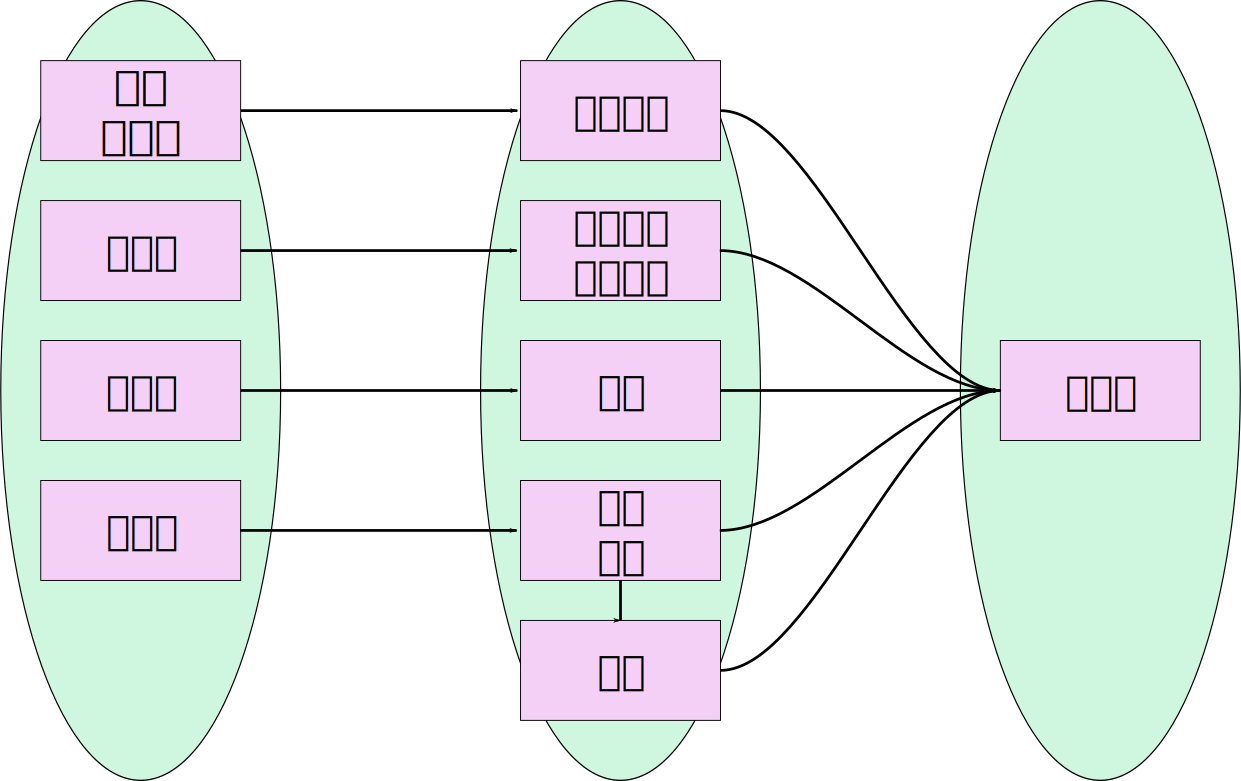
\includegraphics[keepaspectratio,width=40em]{圖/相關研究智識}}
\caption{逐門自然語言處理對應到相關的語言學}
\label{圖:相關研究智識}
\end{figure}

%漢語聲韻學→拼音系統
%語音學→語音合成、辨識
%音韻學→變調
%句法學→斷詞、剖析、翻譯
%語料庫

華語到閩南語的翻譯是自然語言處理(Natural Language Processing)\footnote{人講的話攏是自然語言}的一部份,
佇處理自然語言的時陣就需要語言相關的智識,會當簡單整理做圖\ref{圖:相關研究智識},
無仝的自然語言研究方向,愛知影的語言學智識嘛無仝。
紲落來就介紹語言學佮自然語言處理的研究文獻佮母語的研究狀況:

\section{音標系統}
\label{節:音標系統}
音標系統有兩種,一種是研究語音用的記音系統,一種是予一般人拼寫用的拼音系統。

\subsection{記音系統}
\label{小節:記音系統}
研究一个語言,愛先了解伊的語音,
這時陣就需要一个標準化的記音符號。
這馬上時行的是國際語言學會(International Phonetic Association)制定的
國際音標(International Phonetic Alphabet,IPA)\cite{WIKI國際音標},
毋管記錄的語言有仝款無,只要語音的特徵仝款,就會用仝款的符號。

\subsection{拼音系統}
\label{小節:拼音系統}
記音的音標符號較濟,有的符號是較罕得看著,用起來無方便。
實際寫文章、編教材大部份會用另外的音標系統。
下跤照歷史年代簡單介紹閩南語主要三種拼音系統:

\subsubsection{臺灣閩南語羅馬字拼音}
臺灣閩南語羅馬字拼音是中華民國教育部佇2008年發佈的拼音方案,簡稱做臺羅。
伊的前身是教會羅馬字(白話字)\cite{WIKI教會羅馬字}
佮臺灣語言音標(Taiwan Language Phonetic Alphabet,TLPA)\cite{WIKI臺灣語言音標},
這馬猶原相容教會羅馬字。


\subsubsection{方音符號}
方音符號,又稱方言音符號\cite{華、台語注音符號溯源}
將華語的注音符號閣加一寡聲母、韻母佮聲調符號來標注閩南語。
是1946年朱兆祥教授設計,
佇1998年時,中華民國教育部嘛捌公告使用過。

\subsubsection{通用拼音}
余伯泉教授\ji{⿱毛灬}頭,想欲統一華語、閩南語、客語佮原住民語的拼音系統。
中華民國教育部佇2002年到2008年規定華語通用拼音當做譯音標準。

%\subsubsection{音標比較表}
%國際音標 臺羅 方音 通用 例字


\section{語音學}
\label{節:語音學}

\begin{table}
\caption{元音表}
\label{表:元音表}
\centering
\begin{tabular}{c|ccc}
\diaghead{\theadfont Diag ColumnmnHead II}{喙舌懸低}{喙舌前後}
%喙唇扁/圓 
& 頭前 & 中央 & 後壁\\
\hline
懸 & [i] & [ɨ] & [u]\\
中懸 & [e] &  & [o]\\
中 &  & [ə] & \\
中低 & [ɛ] &  & [ɔ]\\
低 & [a] &  & [ɑ]\\
\end{tabular}
\end{table}

%\begin{table}
%\caption{輔音表}
%\label{表:輔音表}
%\centering
%\begin{tabular}{c|ccc}
%\diaghead{\theadfont Diag ColumnmnHead II}{發音方式}{喙舌所在}
%& 喙唇 & 中央 & 後壁\\
%\hline
%清塞音 & [i] & [ɨ] & [u]\\
%濁塞音 & i & ɨ & u\\
%鼻音 & [e] &  & [o]\\
%邊音 &  & ə & \\
%擦音 & ɛ &  & ɔ\\
%\end{tabular}
%\end{table}

\begin{table}
\caption{音節分析}
\label{表:音節分析}
\centering
\begin{tabular}{cccccc}
字 & 聲母 & \multicolumn{3}{c}{韻母} & 聲調\\
 & & 介音 & 主要元音 & 韻尾 &\\
\tsoo{良}{⿳⿳⿳ㄌㄧㆲˊ}{liong5} & [l] & [j] & [o] & [ŋ] & 5\\
\tsoo{媠}{⿳⿳⿳ㄙㄨㄧˋ}{sui2} & [s] & [u] & [i] & & 2\\
\tsoo{遠}{⿳⿳ㄏㆭ˫}{hng7} & [h] & & [ŋ̩] & & 7\\
\tsoo{意}{⿳ㄧ˪}{i3} & & & [i] & & 3\\
\end{tabular}
\end{table}

語音學(Phonetics)主要討論喙舌的運動方式佮語音的物理性質。

前國際語言學會會長John Ohala捌講過:
「語音變化是連續的(Continuous),為著研究只好假設做離散特徵(Discrete)的音素(Phoneme)。」
可比講「\tsoo{狗}{⿳⿳ㄍㄠˋ}{kau2}」,
音標寫做[kau],
實際上[k]佮[a]、[a]佮[u]中央有誠濟過渡的音,
毋過過渡的音實在傷濟,
無法度一个一个寫出來,
只好用[k]、[a]佮[u]三个符號代表「\tsoo{狗}{⿳⿳ㄍㄠˋ}{kau2}」的音標。

語音會當用氣流有順無,
大略仔分做元音(Vowel)佮輔音(Consonant)。
表\ref{表:元音表}是幾仔个閩南語定用的元音,
會當看著[i]佮[u]攏是喙舌較懸發的音,
而且喙舌佇i發音時比u發音閣較頭前,
這嘛影響著\ji{⿰因}的頻譜(Frequency Spectrum),
[i]佮[u]共振鋒(Formant)嘛小可無仝。
[i]佮[u]喙型嘛無仝,
唸「\tsoo{ㄨ}{}{u}」的時陣喙尖尖,
唸「\tsoo{ー}{}{i}」的時陣喙較平,
嘛影響著語音的變化。
%裂 sai sai:伊笑甲~~~
%裂喙:伊笑的時陣攏會~~

佇分析漢語的時,
會親像表\ref{表:音節分析}仝款,
共音節拆做聲母、韻母佮聲調來看,
韻母閣會當分做介音、主要元音佮韻尾。
毋過愛注意,
這个分析只是方便研究,
聲母、韻母的元素佮聲調猶原會互相影響。


若了解語音學,
就會當知影語音變化的道理,
支持音韻學的理論。

\section{音韻學}
\label{節:音韻學}

\begin{table}
\caption{閩南語上細配對}
\label{表:上細配對}
\centering
\begin{tabular}{c|cc}
& 喙唇 & 中央\\
\hline
元音、鼻化音 & [i](\tsoo{異}{⿳ㄧ˫}{i7}) & [ĩ](\tsoo{院}{⿳ㆪ˫}{inn7})\\
配合濁聲母 & [bi](\tsoo{味}{⿳⿳ㆠㄧ˫}{bi7}) & [mĩ](\tsoo{麵}{⿳⿳ㄇㄧ˫}{mi7})\\
\end{tabular}
\end{table}

現代的音韻學(Phonology)是對Ferdinand de Saussure\cite{de2011course}提出語言學研究,
必須分做共時(Synchronic Phonology)佮歷史(Diachronic Phonology)兩種音韻學。

\subsection{共時音韻學}
\label{小節:共時音韻學}
共時音韻學就是對一个時間的一个語言,
%討論變化,心中所想音檔→唸出來。
討論「頭殼底所想的音」到「唸出來的聲音」的語音變化。
佇討論語音進前,
阮就愛先訂出共時的語音單位,
定用的語音單位是音素。
音素代表一个人「頭殼底」,
對一个語言的「語音單位」。
愛判斷兩个音是毋是仝一个音素,
會當來揣「上細配對」。
可比講表\ref{表:上細配對}第一逝,
一般元音佮鼻化元音會當分出無仝的字,
所以[i]佮[ĩ]對人來講是辨識語音的單位,
是無仝的兩个音素。

\begin{equation}
\label{式:閩南語濁聲母變化式}
B\rightarrow\left\{\begin{matrix}
[b], & 佇一般元音頭前\\ 
[m], & 佇一般鼻化音頭前
\end{matrix}\right.
\end{equation}
\begin{table}
\centering
\caption{閩南語濁聲母無鼻化的選擇}
\label{表:閩南語濁聲母無鼻化的選擇}
\begin{tabular}{c|cc|c}
Bi+無鼻化 & 元音符合鼻音要求 & 規个音節鼻化一致 & 上好的選擇 \\
\hline
{[}bi{]} & & & ←是\tablefootnote{佇優選理論內底,←代表上好的選擇}\\
{[}bĩ{]} & *!毋是\tablefootnote{佇優選理論內底,*代表違反限制,!代表出局} & *毋是\cellcolor{gray}\tablefootnote{佇優選理論內底,殕色底代表選擇出局,毋免比} & \\
{[}mi{]} & & *!毋是 & \\
{[}mĩ{]} & *!毋是 & \cellcolor{gray} & \\
\end{tabular}
\caption{閩南語濁聲母有鼻化的選擇}
\label{表:閩南語濁聲母有鼻化的選擇}
\begin{tabular}{c|cc|c}
Bi+有鼻化 & 元音符合鼻音要求 & 規个音節鼻化一致 & 上好的選擇 \\
\hline
{[}bi{]} & *毋是 & \cellcolor{gray} & \\
{[}bĩ{]} & & *毋是 & \\
{[}mi{]} & *毋是 & *毋是\cellcolor{gray} & \\
{[}mĩ{]} & & & ←是\\
\end{tabular}
\end{table}

毋過看第二逝,
濁輔音佇[i]頭前是塞音[b],
佇[ĩ]頭前是變化鼻音[m],
因為無對比通證明[b]佮[m]有分辨字的能力,
所以[b]佮[m]對人來講「可能」是仝一个語音單位,
會當歸類做一个音素$B$\footnote{這个符號用m、b攏會使,伊只是代表一个音素},
只是$B$佇無仝的所在會唸無仝的音。

音韻學家就想欲揣出「頭殼底所想的音」到「唸出來的聲音」的關係,
討論為啥物面頂的$B$有時唸[b],有時陣唸[m],
目前較大的有衍生音韻學(Generative Phonology)佮優選理論(Optimality Theory)兩大派。

\subsubsection{衍生音韻學}
衍生音韻學是希望揣出的對應音韻規則(Phonological Rule),
親像面頂[b]佮[m]的問題會當看閩南語濁聲母變化規則\ref{式:閩南語濁聲母變化式},
$B$若後壁是一般元音,就變做[b],
若後壁是鼻化音,就變做[m]。

\subsubsection{優選理論}
第二派優選理論是揣出一寡人類語言通用的現象,
而且共這現象,
照重要程度排先後,
去揀人為啥物愛唸這个音。

可比講[b]佮[m]的問題,
阮有「元音符合鼻音要求」佮「規个音節鼻化一致」\cite{yip1996lexicon}兩个現象,
第一个現象「元音符合鼻音要求」是希望主要元音愛符合頭殼內有鼻音無鼻音的條件,
第二个現象「規个音節鼻化一致」是希望音節全部的音素,
\ji{⿰因}鼻化狀況是仝款的,
而且第一个現象比第二个現象優先,
若第一个現象無過,就免比第二个現象。

親像表\ref{表:閩南語濁聲母無鼻化的選擇},
假設頭殼底想的是「Bi+無鼻化」,
阮先產生[bi]、[bĩ]、[mi]、[mĩ]四个選擇\footnote{選擇其實閣有pi、pĩ、…無限濟个,\ji{⿰因}會用別的現象揀掉。為著簡單說明就無寫出來。},
其中[bĩ]佮[mĩ]違反第一个現象,
[bĩ]佮[mĩ]予人揀掉,
[bĩ]、[mi]違反第二个現象,
毋過因為[bĩ]早就違反第一个現象,
無需要閣判斷第二个現象,
所以第二个現象揀掉[mi]
上尾賰[bi],就是上好的選擇。
表\ref{表:閩南語濁聲母有鼻化的選擇}是「Bi+有鼻化」的例,
伊佇第一个現象揀掉[bi]、[mi],
第二个現象揀掉[bĩ],
上尾賰[mĩ]是上好的選擇。

\subsection{歷史音韻學}
\label{小節:歷史音韻學}
\begin{table}
\caption{閩南語低元音提昇過程\cite{hsieh2012low}}
\label{表:閩南語低元音提昇過程}
\centering
\begin{tabular}{ccc}
階段  & 音值 & 來源 \\
Stage 1 & jan/jat\tablefootnote{[i]的介音寫做[j]} &  Doty (1853), dictionary of Amoy dialect\\
Stage 2 & jan/jat &  Luo \& Zhou’s fieldwork in 1930 (L\&Z 1975)\\
Stage 3 & jen/jet & Taiwanese and some Southern Min dialects\\
Stage 4 & en/et & New forms among young Taiwanese speakers\\
\end{tabular}
\end{table}
\begin{equation}
\label{式:閩南語咸攝三等變化式}
[jaC]\rightarrow[jeC]\rightarrow[eC],若C\in\left\lbrace n,t\right\rbrace 
\end{equation}
\begin{equation}
\label{式:閩南語非咸攝三等變化式}
[jaC]\nrightarrow[jeC],若C\not\in\left\lbrace n,t\right\rbrace
\end{equation}
%[ja]\nrightarrow[je]

歷史音韻學是討論語言長期的變化佮語言互相的影響,
這个變化無一定是講話的人講無清楚,
嘛有可能是因為音相倚,
聽話的人聽毋著,
一緣一緣的人沓沓仔改變的。

親像表\ref{表:閩南語低元音提昇過程}記錄
閩南語「\tsoo{先}{⿳⿳ㄒㄧㄢ}{sian1}」佮「\tsoo{節}{⿳⿳⿳ㄐㄧㄚㆵ}{tsiat4}」韻母
這兩百冬的變化,
所以阮會當共這變化整理做規則\ref{式:閩南語咸攝三等變化式}。
除了寫出規則以外,
閣愛需要用語音學解釋為啥物會按呢生,
是因為頭前有介音[j],
喙舌佇較懸較頭前的所在\footnote{元音的所在會當看表\ref{表:元音表}},
後壁[n]佮[t]是舌尖音,
喙舌嘛是佇較懸較頭前的所在\footnote{舌尖音佮[i]、[j]的位較倚,讀者會當唸看覓[in]、[en]佮[an],觀察喙舌的變化},
予原本喙舌較低的[a],
變做喙舌較懸較頭前一寡的[e]。

毋過觀察別的韻煞無這種變化,
親像規則\ref{式:閩南語非咸攝三等變化式},
「\tsoo{閃}{⿳⿳⿳ㄒㄧㆰˋ}{siam2}」、「\tsoo{雙}{⿳⿳ㄒㄧㄤ}{siang1}」猶原是[jam]佮[jaŋ]。
用語音學的角度來看,
干焦頭前介音[j],無後壁的韻尾配合,
無法度予[a]變懸變做[e]。


\section{漢語聲韻學}
\label{節:漢語聲韻學}
聲韻學是研究漢語的歷史語言學,
參考韻冊佮現代漢語方言,
討論方言自古到現代的語音變化佮互相影響。

\subsection{韻冊}
\label{小節:韻冊}

聲韻學的主要研究材料就是韻冊,
韻冊會提供逐个字的聲母、韻母佮聲調資訊,
這就是聲韻學家會當提來推測古早漢語的發音系統的原因。

中國自三國南北朝時就有地區方言的韻冊\footnote{李登《聲類》、呂靜《韻集》},
到宋國官方綜合中國北方佮南方的語音系統的廣韻\cite{2002廣韻注漳州漢音}\cite{2010新校互註宋本廣韻},
廣韻是綜合各地的系統,
伊的聲母、韻母、聲調紀錄佇無仝的漢語方言攏會當用。

\subsection{古早中國語音紀錄}
\label{小節:古早中國語音紀錄}

\subsubsection{反切}
\label{小節:反切}

反切是古代中國用的記音方式,
記錄佇韻冊內底。
反切記音需要記兩个字,
一字代表聲母,一字代表韻母佮聲調,
親像閩南語的「\tsoo{東}{⿳ㄉㄤ}{tang}」會用「\tsoo{端}{⿳ㄉ}{t}」「\tsoo{通}{⿳ㄤ}{ang}」表示。%用「車」?

綜合各地的韻冊,
\ji{⿰因}記錄的反切嘛會當佇無仝的漢語方言用,
除了閩南語的「東」會當切做「端通」
華語的「\tsoo{東}{⿳⿳ㄉㄨㄥ}{}」嘛會當反切做「\tsoo{端}{⿳ㄉ}{}」「\tsoo{通}{⿳ㄨㄥ}{}」。

%\subsubsection{韻}
%\label{小節:韻}

%師詩斯


%狗頭後

%\subsubsection{攝等}
%\label{小節:攝等}


%\subsection{古早漢語推測}
%\label{小節:古早漢語推測}

%嘛因為韻冊的紀錄攏毋是實際發音音值,
%誠濟聲韻學家以語音學佮音韻學的理論,
%參考韻冊佮現代方言,
%來推測古早漢語的發音系統。
%
%ian ien en

%\section{句法學}
%\label{節:句法學}
%句法學就是討論啥物是詞、詞的用法、句型的結構。
%親像
%
%陸儉明


\section{機器學習}
\label{節:機器學習}
自然語言的問題定定非常複雜,
有的時陣無法度揣著規則來解決。
這个時陣就會當共資料交予電腦來判斷。

這節就簡單介紹分類器佮隱性馬可夫模型:

\subsection{分類器}
\label{小節:分類器}
分類器是機器學習的一類研究,
先決定分類器的模型生啥款,
模型內底有誠濟參數,
予伊訓練資料,
訓練資料內底有一堆問題佮對應的答案,
分類器會用輸入訓練資料的問題,
揣出上適合的參數, 
予輸入的問題會當用這參數對應到訓練資料的答案。
等待後壁有新的問題入來時,
分類器會用伊訓練出來的參數來算答案。

定用的分類器模型有
高斯混合模型(Gaussian mixture model,GMM)、
決策樹(Decision Tree,DT)、
支持向量機(Support Vector Machine,SVM)佮
深層學習(Deep learning),
逐个分類器的專長無仝,
應用的所在嘛無仝,
會當看表\ref{表:定用的分類器優缺點}。

\begin{table}
\caption{定用的分類器優缺點}
\label{表:定用的分類器優缺點}
\centering
\begin{tabular}{ccc}
分類器 & 優點 & 缺點 \\
高斯混合模型 & 知影「結果正確」的機率 & 訓練的過程無一定收斂 \\
決策樹 & 輸入會當是字串、符號 & 訓練資料的答案數量愛平均分配\\
支持向量機 & 效果好,效果閣穩定 & 答案的種類無法度傷濟\\
深層學習 & 效果上好 & 訓練資料愛非常濟,使用門檻非常懸\\
\end{tabular}
\end{table}
%\subsubsection{支持向量機}
%\label{小節:支持向量機}
%
%\subsubsection{決策樹}
%\label{小節:決策樹}
%
%\subsubsection{高斯混合模型}
%\label{小節:高斯混合模型}

\subsection{隱性馬可夫模型}
\label{小節:隱性馬可夫模型}
隱性馬可夫模型(Hidden Markov Model,HMM)是針對有狀態轉移的問題,
毋過阮看袂著「狀態」本身,
阮只會當看著佮狀態有關係的「現象」。
隱性馬可夫模型就是想欲用阮看著的現象,
去推測實際的狀態倒底是按怎變化。

%\cite{HMM}
%例


\section{語音辨識}
\label{節:語音辨識}
語音辨識(Speech Recognition)就是共語音轉做文字,
會當用佇語音指令佮問答系統\footnote{親像蘋果公司的Siri}。

語音辨識主要的做法是揣出語音佮音標的對應,
共語音轉做一个一个MFCC聲學特徵,
%\footnote{用MFCC特徵\cite{MFCC特徵}是因為實驗的效果上好\cite{MFCC上好}}
用分類器去判斷是佇一个音標。

因為語音訊號連續閣無固定長度,
為著解決這个問題,
就假設語音變化是狀態的轉移,
用隱性馬可夫模型來模擬語音狀態的變化。

這方面的開源工具有HTK佮Kaldi:

\subsection{HTK}
\label{小節:HTK}
HTK全名號做Hidden Markov Model Toolkit\cite{young2006htk},
發展的時間較早\footnote{對1989年到最近上新的2009年版本},
伊主要用的高斯混合模型當做分類器,
而且用決策樹合併相倚的高斯模型。

%HTK的模型訓練腳本\footnote{會當參考附錄\ref{章:臺灣言語工具}的臺灣言語工具,內底有提共HTK訓練佮使用的腳本},
%一開始會先照文本的音,共音檔平均切做一个一个,
%HTK流程圖~~

%決策樹
%wfst

\subsection{Kaldi}
\label{小節:Kaldi}
Kaldi\cite{Kaldi:Povey_ASRU2011}是較新的工具,
除了訓練一開始嘛是佮HTK仝款用高斯混合模型以外,
伊訓練後壁閣加入深層學習佮其他的演算法,
效果比HTK閣較好。


%SGMM

\section{語音合成}
\label{節:語音合成}
語音合成(Speech Synthesis)是佮文字轉做聲音,佮語音辨識顛倒反。
親像車站廣播,有聲冊攏是語音合成的應用。
這馬時行的做法有模型合成(Model-based Speech Synthesis)佮接音合成(Corpus-based Speech Synthesis)兩種:

\subsection{模型合成}
\label{小節:模型合成}
這个方法揣出音標\footnote{用人工抑是語音辨識軟體標記}佮語音的對應關係,
啥物音標會唸啥物音。
頭一步是用合成器(Vocoder)共語音訊號轉做一个一个的頻譜佮頻率,
才用隱性馬可夫模型佮分類器,
共音標當做輸入,
頻譜佮頻率當作輸出訓練隱性馬可夫模型佮分類器的參數。
等欲合聲音時,才閣照模型的特徵,
用合成器合聲音出來。

伊的輸出語音,
韻律攏誠自然,
毋過聲音的品質比原本語料的音質較\ji{⿰禾黑}一寡,
因為訓練的時,
聲音先用合成器轉做特徵,
合成的時,
特徵閣用合成器轉語音,
兩擺轉換造成音質變\ji{⿰禾黑}。

\subsubsection{HTS}
\label{小節:HTS}
這方面開源軟體有HTS(HMM-based Speech Synthesis System)\cite{hts_zen2007hmm},
伊是對HTK修改來的,
仝款用隱性馬可夫模型、高斯混合模型佮決策樹。
%合成器用SPTK
%用mgc、lf0、duration做聲音特徵,
%
%伊訓練方式,
%伊一个聲音會分做5个state\footnote{下跤講著的5狀態、三連音,攏是參數,毋是固定的},
%逐个state有一个高斯模型,
%伊會先訓練逐个音的初步模型,
%閣來訓練三連音模型,
%閣用決策樹共相倚的音綁做伙。
%
%合的時陣才閣查決策樹,
%共mgc、lf0、duration查出來,
%閣用合成器合語音出來。
%莫用GV

HTS有3000~7000句的訓練語料,
就會當得著袂\ji{⿰禾黑}的效果,
缺點若有聲音效果\ji{⿰禾黑},歹除錯。

%伊需要音檔,標記發音內容的音檔,閣有音類的問題集。設計標仔。
%標仔的時間會使對HTK訓練。
%根據經驗,3000句會使,5000句普通,7000句上好。

\subsection{接音合成}
\label{小節:接音合成}
模型合成有音質的問題,
為著保持音質,
接音合成共原本的音檔庫切做一个一个細音檔,
合成的時陣,
提細音檔來接起來。

對漢語來講,
只需要共逐種音錄起來就好矣,
毋過一字一字聽起來無順無自然。

為著改善接起來韻律無自然的問題,
接音合成會配合模型合成,
用模型產生的韻律,
揀接起來較自然的細音檔。
按呢做的優點是聲音品質誠好,
缺點是語料愛有夠,
因為需要誠濟的細音檔來配合韻律,
若拄著合成品質無好的語句,
就錄音增加音檔庫就好矣。

\subsection{變調佮重音預測}
\label{小節:變調佮重音預測}
佇書寫的音標佮實際唸的發音定定是無仝款的,
上大的差別就是聲調佮重音。
親漢語有聲調,
聲調到發音之間有變調的問題。
南島語有重音,
標註語句的重音嘛是一个音韻學的研究問題。

用閩南語做例,
準做想欲共閩南語的音標變做閩南語的聲音,
毋過實際的音標到唸的發音閣無仝,
後且閩南語的變調傷過複雜的,
需要專門的處理。

楊允言教授就有做過閩南語的變調系統\cite{iunn:台語變調系統實作研究},
用斷詞、詞性佮句型的資訊,
配合20類音韻規則來變調,
得著88.90\%的結果。
音韻規則的優點是語料無蓋濟的時,
就會當得著八九成的正確率,
毋過若數量一濟,
規則的先後會較歹處理。

變調嘛會當用分類器來做,
共規則式用著的特徵當做參數下入去,
看佗一个分類模型會較好。
伊上大的好處就是管理方便,
拄著新語料,重訓練模型就好矣,
缺點是訓練資料需要誠濟。

\subsection{相關系統}
\label{小節:語音合成相關系統}
目前臺灣母語的語音合成只有閩南語佮客話,
親像表\ref{表:語音合成研究、系統},
頭前三个攏是用接音合成,配合字的錄音
第四第五个是接音合成配合韻律模型
上尾一个主要是訓練閩南語HTS模型。

因為南島語的語料較少,
嘛無法度親像漢語幾字仔錄音就有基本的效果,
就需要請專人來錄音、整理,
這是咱閣愛拍拼的所在!

\begin{table}
\caption{臺灣母語語音合成相關研究、系統}
\label{表:語音合成研究、系統}
\centering
\begin{tabular}{ccc}
1999 & 林川傑 & 閩南語翻譯佮語音合成系統\cite{中文到閩南語之線上翻譯及閩南語之語音合成} \\
2002 & 李雪貞 & 客家語語音合成之初步研究\cite{李雪貞2002客家語語音合成之初步研究} \\
2005 & 楊允言、劉杰岳佮李盛安 & 台語羅馬字發音試驗系統\cite{楊允言_台語羅馬字發音試驗系統} \\
2008 & 陳信宏、余秀敏佮羅烈師 & 客語文句轉語音及語音辨認之研究\cite{陳信宏2008客語文句轉語音及語音辨認之研究} \\
2010 & 蔡依玲 & 基於隱藏式馬可夫模型之客語文句轉語音系統\cite{蔡依玲2010基於隱藏式馬可夫模型之客語文句轉語音系統} \\
2013 & 薛丞宏 & 意傳文化科技\cite{意傳文化科技}
\end{tabular}
\end{table}

\section{斷詞}
\label{節:斷詞}
斷詞是共語句照一个詞一个詞分開的技術,
親像漢語佮日語的文字定定是一字一字無分開,
就看袂出來倒底佗一字佮佗一字是一个詞,
若愛提著詞的資訊,
就需要程式來斷詞。
斷詞的效果嘛會影響著翻譯、變調佮其他技術的效果。

有一寡語言現象是佮詞有關係,
親像閩南語的變調,
毋過漢語語句的文本,

所以就需要斷詞,
共詞佮詞分開,
後壁的應用才有法度繼續落去。



%轉格式
%斷詞前
%自稱一世人離袂開預報工作的吳德榮
%tsu7 tshing1 tsit8 si3 lang5 li5 be7 khui1 ...
%斷詞後
%自稱 一世人 離袂開 預報 工作 的 吳德榮
%tsu7-tshing1 tsit8-si3-lang5 li5-be7-khui1 ...


華語這方面有中研院中文斷詞系統(CKIP)\cite{CKIP論文}。

閩南語斷詞的標準,
自誠早以前就有人討論矣\cite{台語斷詞原則討論},
教育部嘛有出「臺灣閩南語羅馬字拼音方案連字符使用原則」\cite{臺羅拼音},
定義連字符的標準。

%斷詞的標準有誠濟種,為著方便,以教育部的「臺灣閩南語羅馬字拼音方案連字符使用原則」的連字符當做一个詞,若「tsiah8 png7」(食白米飯的意思),當做兩个詞,「tsiah8-png7」(食物件的意思),當做一个詞。


%斷詞方法:長詞優先、配合語言模型、統計式、馬可夫、詞性

\subsection{長詞優先斷詞}
\label{節:長詞優先斷詞}

定看著的斷詞方法有長詞優先(Maximum Matching),
伊的做法是自後頭開始看\footnote{華語實驗的結果,自後頭開始的效果比對頭前的閣較好},
往頭前幾个字是毋是會當揣著一个佇辭典的詞,
若會使,就揀上長的彼个,
希望詞愈長愈好,會當看方法\ref{方法:長詞優先斷詞方法}。

%解釋比如說,『我想要吃飯』可以切成『我,想,要,吃,飯』『我,想要,吃飯』『我,想要吃飯』『我想要,吃飯』『我想要吃飯』,其中,能夠在字典找到詞的切割方式有『我,想,要,吃,飯』『我,想要,吃飯』,

\begin{algorithm}
  \caption{長詞優先斷詞方法}
  \label{方法:長詞優先斷詞方法}
  \begin{algorithmic}
    \REQUIRE 無斷詞的語句$[j_{1}, j_{2}, ... , j_{m}]$
    \ENSURE 斷詞的語句$[s_{1}, s_{2}, ... , s_{n}]$
    \STATE \( 決定辭典上長的詞字數$k$ \)
    \STATE 揣一个上細的\(i\),予\(j_{i+1}, j_{i+2}, ... , j_{m}\)是辭典的一个詞,而且\(m − k ≤ i ≤ m − 1\)
    \STATE 斷詞的語句加入\(s=j_{i+1}, j_{i+2}, ... , j_{m}\)
    \STATE \( $m=i$ \),重做第1步,到\(i=0\)為止
  \end{algorithmic}
\end{algorithm}


%\section{詞性標記}
%\label{節:詞性標記}
%\subsection{相關系統}
%\label{小節:詞性標記相關系統}
%\cite{iunn:利用統計方法及中文訓練資料處理台語文詞性標記}
%

\section{剖析}
\label{節:剖析}
剖析是了解語句內底詞的關係,
分析語句的句型。
剖析會當用佇翻譯佮語意分析,
較定看著的就是問答系統\footnote{親像蘋果公司的Siri}。

做剖析需要句法學的知識,
閣愛有一致的人工檢查,
這是一个誠大的工程。

%http://nlp.stanford.edu/software/stanford-dependencies.shtml#Download
%http://stackoverflow.com/questions/10401076/difference-between-constituency-parser-and-dependency-parser
\subsection{相關系統}
\label{小節:剖析相關系統}
楊允言教授捌做過閩南語的剖析樹仔\cite{台語文語法結構樹建置},
毋過數量猶原無夠,需要閣整理。

一開始的語料歹收集,
有一个辦法是借用華語的剖析,
先共閩南語翻譯做華語,
才閣共華語語句的剖析樹仔\cite{chen2005chinese}對應去閩南語語句,
按呢就有初步的樹仔矣。
訂好剖析樹仔規則了後,
就會使整理初步的樹仔,
等待資料有夠濟,
就會提樹仔的語料來訓練一个閩南語的剖析器\cite{klein2003accurate}。

%人工若校對,全部的資料著愛收集起來
%而且嘛愛親像XX節的XX圖仝款,愛做一个改錯誤的程式,予人工莫一直改仝款的物件
。

\section{翻譯}
\label{節:翻譯}
這馬電腦時行的翻譯方式是統計式機器翻譯(Statistical Machine Translation),
這是對1993年Brown用數學證明\cite{brown1993mathematics}開始,
一直發展到這馬。
統計式機器翻譯會當分做對齊模型(Alignment Model)、語言模型(Language Model)佮解碼器(Decoder)三个部份:

\subsection{對齊模型}
\label{小節:對齊模型}
對齊模型的功能是予解碼器知影詞愛按怎翻譯,
可比講是一个雙語的辭典。

對齊模型有分斷詞對齊佮剖析樹對齊兩種,下跤用斷詞對齊說明伊的原理。

先準備一組一組的華語閩南語平行語料,
親像「我 要 吃飯」和「我 欲 食 飯」,
紲落來產生語詞對照表。
華語詞的「要」,會對應到「我」、「欲」、「食」、「飯」閩南語詞,
經過大量的平行語料,
上尾知影華語的「要」定定對應著閩南語的「欲」,
也就是共對應頻率懸的組合留落來。
%改例

開源工具GIZA++\cite{och2003systematic}實作Brown 1993的演算法,
而且這馬嘛有支援多核心的MGIZA\cite{gao2008parallel}。

\subsection{語言模型}
\label{小節:語言模型}
第二部份是語言模型(language model),伊是欲用來判斷一句話是好是\ji{⿰禾黑}。

%加數學解釋
伊的做法是去記錄逐个詞後壁定定會接啥物詞,
若有一句話是「…欲 食…」,有「欲」佮「食」兩个詞,
咱知影「…欲 食」的後壁接「飯」比「…欲 食」的後壁接「湯」的機率較大,
也就是講「欲 食 飯」連紲詞比「欲 食 湯」連紲詞機率大,
若語言模型一擺看「欲 食 飯」三个詞,
就是三連紲詞模型(3-grams model)。
語言模型判斷一句話,伊出現的機率有偌大,就是看這句話伊內底連紲詞的機率是偌大。
%改例

這方面的工具有IRSTLM\cite{federico2008irstlm}、
SRILM\cite{stolcke2002srilm}佮
KenLM\cite{Heafield-estimate},
其中IRSTLM佮KenLM是LGPL開放授權,
SRILM是學術授權。

\subsection{解碼器}
\label{小節:解碼器}
上尾一部份是解碼器,
提面頂講的對齊模型、語言模型,
來翻譯華語到閩南語。

因為翻譯的問題毋是多項式時間(NP problem)會當解出來的,
所以解碼器袂使硬算全部的可能,
必須用有效率的演算法來翻譯。

上有名的開源程式就是Moses\cite{Koehn:2007:MOS:1557769.1557821},
伊整合對齊模型佮語言模型的介面,
閣有專工的訓練包通使用\cite{Moses訓練包}。

\subsection{評分方式}
\label{小節:評分方式}

翻譯大部份攏用BLEU(Bilingual Evaluation Understudy)來評分,
伊用連紲詞的概念來評分,
$BLEU=100\times{e^{\max{0,\frac{\textit{結果-答案長度}}{\textit{結果長度}}}}}\times{\sum_{n=1}^{4}(\textrm{n連紲詞})^{\frac{1}{4}}}$\cite{BLEU程式}。
%改cite

準若翻譯的答案是「這 幾 工 寒流 閣再 展威」,咱有兩个翻譯的結果,翻譯結果一「這 幾 工 寒流 有 展威」佮結果二「寒流 這 幾 工 閣再 展威」,請看表\ref{表:範例BLEU分數},答案有「這 幾 工」、「幾 工 寒流」、「工 寒流 閣再」佮「寒流 閣再 展威」4个三連紲詞,結果一有出現2个,所以結果一的三連紲詞分數是2/4,結果二有出現1个,分數是1/4。因為結果二無對應的四連紲詞,伊的分數都比結果一低。

\begin{table}
\caption{翻譯結果一「這 幾 工 寒流 有 展威」佮翻譯結果二「寒流 這 幾 工 閣再 展威」對答案「這 幾 工 寒流 閣再 展威」的分數}%
\label{表:範例BLEU分數}
\centering
\begin{tabular}{|c|cccc|c|}
\hline
翻著的數量 & 一連紲詞 & 兩連紲詞 & 三連紲詞 & 四連紲詞 & BLEU分數\\
\hline
結果一 & 5/6 & 3/5 & 2/4 & 1/3 & 53.73\\
\hline
結果二 & 6/6 & 3/5 & 1/4 & 0/4 & 0.00\\
\hline
\end{tabular}
\end{table}

\section{語料收集整理}
\label{節:語料收集整理}
%佇這个網路的時代,收集語料上緊的方法就是去網路面頂掠。看圖XX,先共閩南語專門的字詞擲去搜尋引擊\footnote{親像Google、Bing},閣照揣著的網頁去掠相關的閩南語。
%閩南語的網頁內底除了閩南語以外,有可能閣濫一部份的華語,為著莫予華語語料影響著閩南語模型,所以愛想辦法共臺華兩種語言分開。分開了後
%
%%圖:關鍵詞 引擊 網址 掠網頁 網頁html 轉文字 一句一句的語料 判斷語言 閩南語/華語 對齊
%
%\begin{figure}
%\centerline{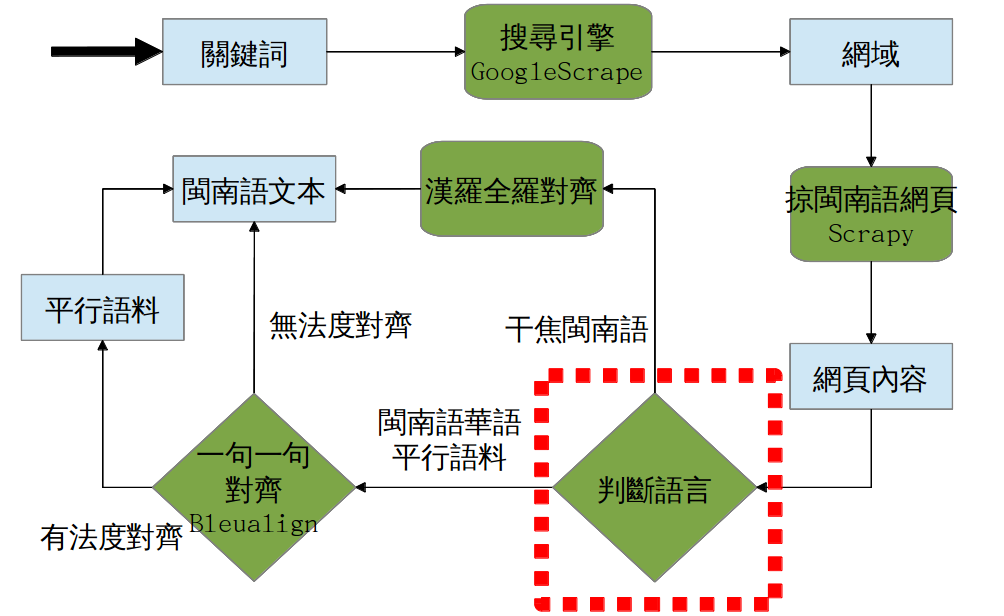
\includegraphics[keepaspectratio,width=40em]{圖/網路語料庫結構}}
%\caption{網路語料庫}
%\label{圖:網路語料庫結構}
%\end{figure}
%
%\subsection{收集網路資料}
%\label{小節:收集網路資料}

\subsection{語言分類}
\label{小節:語言分類}
語言分類(Language Identification)是輸入一句話,
判斷是佗一種語言。
這馬上時行的方法是以字元為單位,語言模型算分數\cite{cavnar1994n}

南島語主要嘛是拼音文字,
所以會使用這个方法,
南島語佮漢語的語言分類較簡單,
就算漢語用羅馬拼音,
拼音的種類嘛差誠濟,
只要檢驗有聲調抑是拼音規則就會使判斷是南島語抑是漢語。

\subsection{平行語料語句對齊}
\label{小節:語句對齊}
翻譯語料的平行語料需要一句一句對齊,
若原本的語料是一篇一篇對應的,
就需要平行語料語句對齊(Parallel Corpus Sentences Alignment)。

語句對齊的方法有誠濟種,
有照字元數量對齊的Gale and Church算法\cite{gale1993program},
嘛有用翻譯結果輔助的Bleualign\cite{zora38464}。

\section{語料庫}
\label{節:語料庫}
自然語言處理需要語料才有法度訓練模型,
就需要語料庫共語料存起來。

\begin{table}
\caption{自然語言處理技術需要的語料庫}
\label{表:自然語言處理技術需要的語料庫}
\centering
\begin{tabular}{lc}
技術 & 語料樣式 \\
變調 & 原始文本、本調音標佮變調音標 \\
語音辨識 & 濟人音檔佮對應文本 \\
語音合成 & 孤人音檔佮對應文本 \\
斷詞 & 斷詞的語料 \\
剖析 & 剖析樹 \\
翻譯 & 兩種語言的平行語料 \\
\end{tabular}
\end{table}

有的語料庫是純文字的資料庫,
嘛有存音檔的語料庫,
愛看需求,定看著的技術會當參考表\ref{表:自然語言處理技術需要的語料庫}。

\subsection{閩南語語料種類}
\label{節:閩南語語料種類}

\begin{table}
\caption{閩南語語料種類比較表}
\label{表:閩南語語料種類比較表}
\centering
\begin{tabular}{lcc}
種類 & 範例 & 備註\\
全漢 & 我欲食飯 & 全部漢字\\
全羅 & gua2 beh4 tsiah8-png7 & 全部羅馬拼音,有斷詞資訊\\
漢羅 &我beh4食飯 & 漢字拼音濫咧用\\
\end{tabular}
\end{table}

閩南語是漢語的一支方言,
大部份的字攏會當揣著漢字,
毋過閩南語嘛毋是純漢語,
有的字無對應的漢字。

有的人慣勢全部用羅馬拼音創作,
這種寫法號做「全羅」。
嘛有人慣勢全部用漢字創作,
號做「全漢」
毋過有的字無法度揣著對應的漢字,
全漢實際上的拄著造字、揣字的困難,
為著創作方便,
知影的字用漢字寫,
賰的用音標寫落來,
號做「漢羅」。
詳細會當看表\ref{表:閩南語語料種類比較表}的範例。

\subsection{閩南語語料-新聞語料庫}
\label{節:新聞語料庫}
iCorpus臺華平行新聞語料庫(後壁用「新聞語料庫」稱呼)\cite{iCorpus臺華平行新聞語料庫}
是中央研究院資訊所陳孟彰老師主持,內底的文章主要是何澤政翻譯的。

何澤政\footnote{一九七零年代出世,臺中烏日人}對民國九十七年十一月初六開始,
逐工揣兩篇華語新聞,先人工斷詞斷句,
後尾翻譯做閩南語教會全羅,
罕得改變用詞的先後。

親像原本的新聞「這幾天寒流再度發威」,翻譯做「tsit4-kui2-kang han5-liu5 koh-tsai3 tian2-ui」(這幾工寒流閣再展威)\footnote{原文是教會羅馬字,為著文章一致,以教育部的臺羅書寫}。
%新聞語料庫的翻譯,親像面頂的「這幾天寒流再度發威」,較袂翻做「寒流這幾工閣再展威」,除非照華語用詞先後翻譯的結果無順,才會調整。

澤政佇語料內底用
「挕捒 hinn3-sak4」%轉格式
\footnote{挕捒意思共物件擲掉、放捒,嘛就是華話的「丟棄」
%,例句甲(家己做的):這支筆好好,為啥物愛共伊挕捒。
%例句乙(Tek-hôa,Nah ē teh批判民進黨?,\url{http://taioan-chouhap.myweb.hinet.net/089.htm}):民進黨接續李登輝的路線, 繼續加強黨國時代權力者, 倚附者佮既得利益者的優勢,毋是共刜挕捒。
}
、
「作孽tsok4-giat8」%轉格式
\footnote{
%青-少-年|tshing1-siau3-lian5 作-孽|tsok4-giat8 跤-踏-車|kha1-tah8-tshia1 擲|tan3 落|loh8 河-中|ho5-tiong1。
%拄著外來詞,澤政嘛會選擇保留原文,拄著華語的「歐巴馬」佮「西藏」,會翻轉去英文「Obama」、「Tibet」。
%愛耍手賤,華語的「惡作劇」。例句甲:叫你莫摸你閣摸,誠實手賤愛作孽!(家己做的)例句乙:你這个作孽囡仔,你是按怎沐甲一身軀烏趖趖?(惠光,天真瀾漫,\url{http://ip194097.ntcu.edu.tw/nmtl/DADWT/thak.asp?id=992})
}
本土的詞以外,伊嘛會配合這馬發生的代誌,用較時行的閩南語,親像
「喙罨」\footnote{華語的「口罩」}、%轉格式
「心肌梗窒心|sim1 肌|ki1 梗|king2 窒|that4」\footnote{華語的「心肌梗塞」}、%轉格式
「自來水」\footnote{閩南語較古典的用法,會號做「水道水」}、…。%轉格式

而且除了現代閩南語,澤政伊閣會去查台華線頂辭典\cite{台華線頂辭典}
選擇較古典的用詞\footnote{台華線頂辭典是古早語料,一个詞若台華線頂辭典查有,教育部辭典查無,就當做伊是較古典的詞},親像
「𤺪|sian7 篤-篤|tauh4-tauh4」%轉格式
%\footnote{熱-天|juah8-thinn1 高-溫|ko1-un1 炎-熱|iam7-juah8 規-工|kui1-kang1 𤺪|sian7 篤-篤|tauh4-tauh4 。|。}
、
「鬥-贊-手|tau3-tsan3-tshiu2」。%轉格式
%\footnote{佇|ti7 三|sam1 一-一|it4-it4 大-地-動|tua7-te7-tang7 慷-慨|khong2-khai3 鬥-贊-手|tau3-tsan3-tshiu2 ,|,}。
拄著外來詞,澤政嘛會選擇保留原文,
拄著華語的「歐巴馬」佮「西藏」,
會翻轉去英文「Obama」、「Tibet」。

%若源頭是日本話外來詞,就會直接用教羅寫出來,請看

\subsection{閩南語語料-教育部辭典}
\label{節:教育部辭典}
教育部辭典全名「臺灣閩南語常用詞辭典」\cite{教育部臺灣閩南語常用詞辭典},
正式版是100年上線,
伊有25892的詞條\footnote{1021230的資料},
內底誠濟生活的用語,
大部份詞條攏有漢字、音標、解釋、例句佮翻譯。

這个辭典是教育部編的,當然漢字有照教育部家己的規範\footnote{臺灣閩南語推薦用字700字表,佇96~99年公佈修正}來寫,所以伊內部的用字前後有一致,為著翻譯的效果佮使用者的方便,就共教育部辭典的用字當做標準,若有用字佮教育部的用字無仝的,就改做教育部的用字。%//閣愛順過

伊的例句,除了閩南語漢字佮音標以外,閣有敆華語的翻譯,親像表\ref{表:教育部辭典例句},漢字佮音標的對應會使提去做用字參考的字典,音標的部份會當提來斷詞,訓練語言模型,閩南語佮華語的對應會使提來做平行語料。
嘛因為伊有漢字佮音標,就會當共遮的漢字佮音標收集起來,當做用字參考的字典,
\begin{table}
\caption{教育部辭典例句}
\label{表:教育部辭典例句}
\centering
\begin{tabular}{l}
彼个查某囡仔真媠。 \\
Hit ê tsa-bóo gín-á tsin suí.\\%轉格式
那個女孩子很漂亮。\\
\end{tabular}
\end{table}

除了一般的詞條以外,教育部辭典嘛有收一寡俗語、臆謎猜,攏做388句做附錄句。
因為附錄句干焦提供解釋,所以無法度提來做平行語料,毋過會使提來訓練語言模型。


\subsection{閩南語語料-臺文典藏}
\label{節:臺文典藏}
台語文數位典藏資料庫(下跤號做臺文典藏)\cite{台語文數位典藏資料庫}
是國家臺灣文學館收集1885~2006年的語料。
臺文典藏的來源語料百百款,攏總2167篇,
照時代分做清國時期170篇、日治時代490篇,民國統治1507篇。
內底嘛有照語料形式分做四類,有詩387條、散文1127篇、小說387篇、劇本49篇。%攏總416343句。

因為伊是百外冬的語料庫,較古早的語料,用詞就較古典,
格式嘛無仝,有的是漢羅,有的是全羅。
臺文館\ji{⿰因}因為著格式統一,
就替原底是全漢抑是漢羅的語料補全羅拼音\footnote{有時陣劇本邊仔的解釋會用漢字,親像「(福哥仔出場)」}。
若原本是全羅,就請人拍漢羅,會當看表\ref{表:臺文典藏語料},
拍漢羅的時,\ji{⿰因}若知影漢字,就會拍漢字,
賰的外來語,抑是較本土的語詞就會用音標來拍。
伊有的語料是一句對齊一句,有的是一段對齊一段。

\begin{table}
\caption{臺文典藏語料漢羅、全羅對照}
\label{表:臺文典藏語料}
\centering
\begin{tabular}{l}
漢羅:Koh m7知u7危險.........., \\
全羅\footnote{臺文典藏內底原本是教會羅馬拼音,為著讀者方便,攏改做教育部的臺羅}:Koh m7-tsai u7 gui5-hiam2...............,\\
\end{tabular}
\end{table}


\subsection{閩南語語料-TGB通訊臺灣組合}
\label{節:TGB通訊-臺灣組合}
TGB通訊\cite{TGB通訊}是學生台灣語文促進會
對1999年10月開始\cite{學生台灣語文促進會對1999年10月開始}\footnote{\url{}}
一個月一期的刊物。
頭前60期以閩南語為主,61期後有提供華語對照,
有時陣閩南語句內底會濫一寡華語詞,形式較無固定。


%因為有閩南語、有華語佮臺華平行語料,嘛閣有濫做伙的, 誠濟種實際會拄著的情形會當提來做判斷語言的語料。
%有的時陣閩南語佮華語濫做伙,先定義啥物情形算閩南語,啥物情形算華語

%用人工分
%
%主要語句是閩南語,有一兩个詞是華語嘛是算閩南語
%閩南語
%
%聽人講 khah 早有出現過『小蜜蜂』
%我 beh tńg 來種作 ! ── 記 0312 Truku 反亞泥 ‧ 還我土地運動
%有台灣味 ê 繪本──《我和我的腳踏車》 .
%
%華語
%華語閩南語攏通的算華語
%有華語完整的一句話就算華語
%毋是華語嘛毋是閩南語,親像英文、日語、…
%
%「 糟了 ,是工地火燒厝, 緊轉去打 火 ! 」建設公司 的 工地主任 從手機接到消息,通話結束後就帶著那群混混先離開了。
%『聽說妳最近遇到什麼問題 , 是不是 ? 怎麼了 ? 』好性地 ê QA 繼續問--落-去 .
%去越南胡志明市 4 工/越南胡志明市四日行 @Gio̍k-hōng

%\subsection{閩南語語料腔口統計佮處理}
%\label{小節:閩南語語料腔口統計佮處理}




